\chapter{CTMQC applied to the Tully Models}
\label{chap:tully_models}

The Tully models, first proposed by John Tully in 1990 \cite{tully_molecular_1990}, are a collection of model systems. They were designed to be simple enough to obtain accurate quantum results to benchmark new nonadiabatic molecular dynamics (NAMD) methods against. Originally there were 3, 1 dimensional, 1 atom models. However, in this work an extra model has been introduced with parameters taken from Gossel, 18 \cite{gossel_coupled-trajectory_2018}. This is to allow a full comparison of my implementation of CTMQC with the literature. In this chapter my implementation of CTMQC will be tested using these model systems and by comparing my results with those in the literature.
\\\\
In each of the Tully models the (diabatic) Hamiltonian is defined by the nuclear positions and is a 2$\times$2 matrix that takes the form:
\begin{equation}
  \hat{H} = \frac{\ \hat{P} ^2}{2M} + \left(
                                              \begin{array}{cc}
                                                H_{11}(\mathbf{R}) & H_{12}(\mathbf{R}) \\
                                                H_{21}(\mathbf{R}) & H_{22}(\mathbf{R})
                                              \end{array}
                                         \right)
\end{equation}
The nuclear mass is set to 2000 a.u., this was set to be very close to the proton's mass of 1836 a.u. so we can expect significant quantum effects that classical theory couldn't replicate. The values of the Hamiltonian elements are set to produce systems that resemble common features in a typical nonadiabatic simulation such as avoided crossings and regions of extended coupling. The parameters used in each systems' Hamiltonian where taken from Gossel, 18 \cite{gossel_coupled-trajectory_2018} in order to compare the 2 implementations. These can be found in appendix \ref{app:tully_params}.
\\\\
In order to propagate dynamics in the adiabatic basis we need to calculate various quantities from the hamiltonian at each timestep. These are, for Ehrenfest, the (adiabatic) nonadiabatic coupling vector ($\mathbf{d}_{lk}^{(I)}$) and the adiabatic energies ($E_{l}^{(I)}$). In the full CTMQC simulations we must also calculate the adiabatic momentum term $\mathbf{f}_{l}^{(I)}$ from the Hamiltonian. The adiabatic energies are the eigenvalues of the Hamiltonian. The adiabatic NACV can be calculated via an (explicit Euler) finite difference method and equation \eqref{eq:NACV_def} below.
\begin{equation}
  \mathbf{d}_{lk}^{(I)} = \langle \psi_{l}^{(I)} | \nabla \psi_k^{(I)} \rangle
  \label{eq:NACV_def}
\end{equation}
Where $\psi_{l}^{(I)}$ is the adiabatic electronic basis function. This is given by the eigenvector of the Hamiltonian, on replica I, corresponding to state l. Illustrations of these 2 properties can be found below in fig \ref{fig:tully_schematics} for each of the 4 models systems.
\begin{figure}[H]
  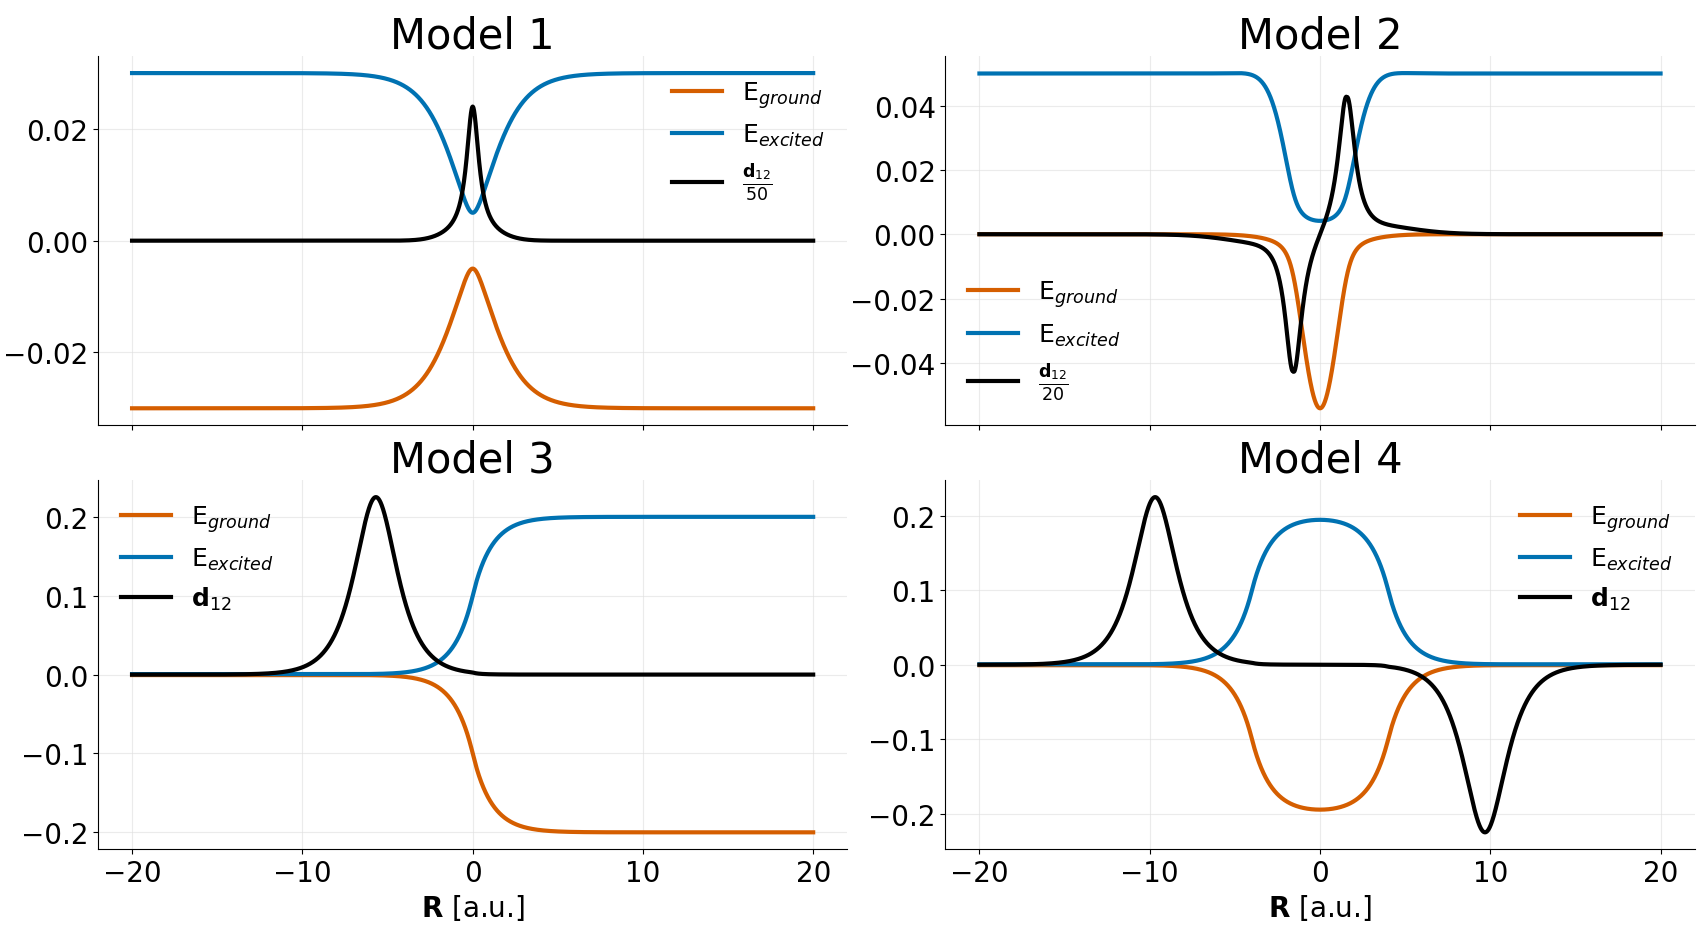
\includegraphics[width=\textwidth]{Chapter_tullyModels/model_schematics.png}
  \caption{\label{fig:tully_schematics}Adiabatic potential energy surfaces (orange and blue) and element 1, 2 of the nonadiabatic coupling vector (black) for the 4 model systems. For parameters see appendix \ref{app:tully_params}.}
\end{figure}
\newpage
\noindent In order to initialise the simulations coordinates and velocities were sampled from the Wigner phase-space distribution of a gaussian nuclear wavepacket given by equation \eqref{eq:initial_nucl_wp}. A derivation of this can be found in appendix \ref{app:Wigner}.
\begin{equation}
  \chi(R, 0) = \frac{1}{(\pi \mu^2)^{\frac{1}{4}}} e^{-\frac{(R - R_0)^2}{2 \mu^2} + \im k_0 (R - R_0) }
  \label{eq:initial_nucl_wp}
\end{equation}
The adiabatic coefficients were intialised purely on the ground state and the initial width of the nuclear wavepacket was set to $\mu = \sqrt{2}$ bohr. 2 values of initial momenta $k_0$ were chosen for each model, 1 low value and another higher one. Full details of all input parameters can be found in appendix \ref{app:tully_params}.
